\begin{figure}[H]
\centering
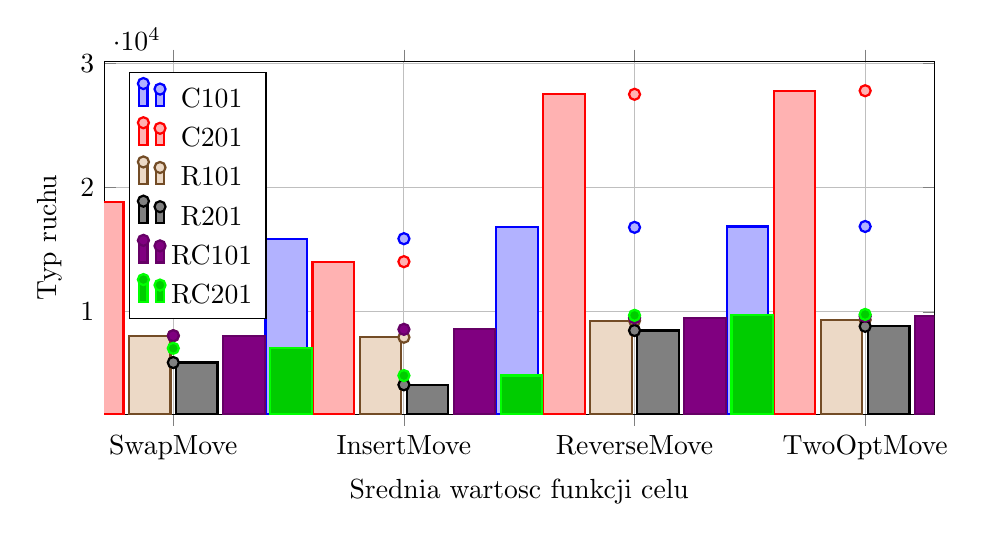
\begin{tikzpicture}
\begin{axis}[
xlabel = {Srednia wartosc funkcji celu},
ylabel = {Typ ruchu},
legend pos = north west,
grid = both,
width=1\linewidth,
height=0.5\linewidth,
ybar,
bar width=15pt,
symbolic x coords={SwapMove,InsertMove,ReverseMove,TwoOptMove,},
xtick=data
]
\addplot + [mark = *, thick] coordinates
    {
(SwapMove,14607.0)(InsertMove,15891.0)(ReverseMove,16806.0)(TwoOptMove,16876.0)};
\addlegendentry
{C101}
\addplot + [mark = *, thick] coordinates
    {
(SwapMove,18845.333333333332)(InsertMove,14040.666666666666)(ReverseMove,27524.333333333332)(TwoOptMove,27810.0)};
\addlegendentry
{C201}
\addplot + [mark = *, thick] coordinates
    {
(SwapMove,8074.333333333333)(InsertMove,7952.666666666667)(ReverseMove,9285.333333333334)(TwoOptMove,9352.0)};
\addlegendentry
{R101}
\addplot + [mark = *, thick] coordinates
    {
(SwapMove,5916.333333333333)(InsertMove,4123.666666666667)(ReverseMove,8496.666666666666)(TwoOptMove,8834.0)};
\addlegendentry
{R201}
\addplot + [mark = *, thick] coordinates
    {
(SwapMove,8074.0)(InsertMove,8589.666666666666)(ReverseMove,9511.0)(TwoOptMove,9642.666666666666)};
\addlegendentry
{RC101}
\addplot + [mark = *, thick] coordinates
    {
(SwapMove,7063.0)(InsertMove,4865.0)(ReverseMove,9719.333333333334)(TwoOptMove,9789.666666666666)};
\addlegendentry
{RC201}
\end{axis}
\end{tikzpicture}
\caption
{Srednia wartosc funkcji celu w zaleznosci od typu ruchu dla poszczegolnych instancji}
\label{fig:mean_goals_per_move_type_per_instance}
\end{figure}
